\section{求解结果的误差与可信程度}
\label{sec:ls-numerical-sensitivity}

求解目标确定以后，还要回答算出的结果能相信多少。本节分三方面讨论：数据的扰动怎样传到解，算出的近似解怎样用残差判断，矩阵的秩变化时伪逆怎样变化。讨论每种误差都先说清以什么为参照、允许修改哪些数据：比较两个精确解时修改的是$\bm A$或$\bm b$；用残差判断近似解时数据不改，参照的是未知的真解；后向误差则反过来问数据至少要改多少，近似解才成为精确解。以下结论都由精确方程、范数估计和奇异值性质建立，扰动可以有有限大小；第~\ref{chap:multivariate-calculus}章再从同样的精确关系中提取局部线性响应。

\subsection{右端项与系数矩阵的有限扰动}
\label{sec:ls-equation-sensitivity}

本小节设$\bm A\in\mathbb R^{d\times d}$可逆，$\bm b\ne\bm0$，精确解$\bm x_\star=\bm A^{-1}\bm b$。向量范数与它诱导的矩阵范数始终取同一种，记$\kappa(\bm A)=\lVert\bm A\rVert\lVert\bm A^{-1}\rVert$。

\paragraph{右端扰动}
先固定$\bm A$，只把右端改为$\bm b+\Delta\bm b$。两个方程相减，解的变化$\Delta\bm x=\bm A^{-1}\Delta\bm b$对任意大小的$\Delta\bm b$都精确成立。取范数得$\lVert\Delta\bm x\rVert\leq\lVert\bm A^{-1}\rVert\lVert\Delta\bm b\rVert$，再用$\lVert\bm b\rVert\leq\lVert\bm A\rVert\lVert\bm x_\star\rVert$得到相对误差界
\[
 \frac{\lVert\Delta\bm x\rVert}{\lVert\bm x_\star\rVert}\leq\kappa(\bm A)\,\frac{\lVert\Delta\bm b\rVert}{\lVert\bm b\rVert},
\]
这就是第~\ref{sec:ls-matrix-condition-number}节的条件数界（定理~\ref{thm:matrix-analysis-condition-number-bound}）。哪些右端误差放大得最多，可以由奇异值分解$\bm A=\sum_i\sigma_i\bm u_i\bm v_i^\top$读出：把$\Delta\bm b$展开为$\sum_i\beta_i\bm u_i$，就有$\Delta\bm x=\sum_i(\beta_i/\sigma_i)\bm v_i$，沿$\bm u_i$的误差被放大$1/\sigma_i$倍，落在最小奇异值方向上时放大最多。下面的例子都在精确算术中计算，放大完全来自问题本身，与算法和舍入无关。

\begin{example}[良态矩阵与近平行列矩阵]
\label{ex:ls-rhs-perturbation-near-parallel}
取$\bm A_1=\operatorname{diag}(2,1)$，$\kappa_2(\bm A_1)=2$。右端由$(2,1)^\top$改为$(2,1.01)^\top$，解由$(1,1)^\top$变为$(1,1.01)^\top$，右端与解的相对变化分别约为$0.0045$与$0.0071$，放大约$1.6$倍。

再取两列接近同向的
\[
 \bm A_2=\begin{bmatrix}1&1\\0&\varepsilon\end{bmatrix},\qquad\varepsilon=10^{-2}.
\]
$\bm A_2^\top\bm A_2$的迹为$2+\varepsilon^2$、行列式为$\varepsilon^2$，所以$\sigma_{\max}\approx\sqrt2$，$\sigma_{\min}\approx\varepsilon/\sqrt2$，$\kappa_2(\bm A_2)\approx2/\varepsilon=200$。右端由$(2,0)^\top$改为$(2,0.01)^\top$，解由$(2,0)^\top$变为$(1,1)^\top$：右端的相对变化为$0.005$，解的相对变化约为$0.707$，放大约$141$倍。解的变化$(-1,1)^\top$几乎正沿着小奇异值对应的右奇异方向，两个系数此增彼减，图~\ref{fig:matrix-analysis-coefficient-sensitivity}画出了$\varepsilon$减小时这种分裂怎样加剧。
\end{example}

\begin{figure}
 \centering
 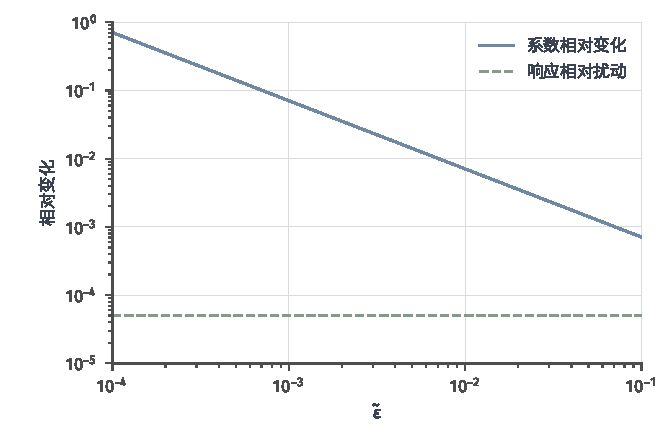
\includegraphics[width=0.92\linewidth]{figures/00-shared/mathematical-preliminaries-upper/02-linear-spaces/matplotlib/matrix-analysis-coefficient-sensitivity/figure.pdf}
 \caption{近平行列的系数分裂：对$\bm A_2=\left[\begin{smallmatrix}1&1\\0&\varepsilon\end{smallmatrix}\right]$固定右端扰动$\eta$，$\varepsilon$越小，两个系数
 沿相反方向偏离$(2,0)$越远，绝对误差随$1/\varepsilon$增长。}
 \label{fig:matrix-analysis-coefficient-sensitivity}
\end{figure}

\paragraph{系数矩阵的扰动}
\label{sec:ls-inverse-sensitivity}%
系数矩阵也带误差时，扰动后的矩阵$\bm B=\bm A+\bm E$甚至可能不可逆，所以要先确定它何时可逆，再估计$\bm B^{-1}$离$\bm A^{-1}$多远。

\begin{theorem}[逆矩阵的有限扰动]
\label{thm:ls-inverse-finite-perturbation}
设$\bm A\in\mathbb R^{d\times d}$可逆，$\bm B=\bm A+\bm E$。
\begin{enumerate}
 \item 若$\lVert\bm A^{-1}\bm E\rVert<1$，则$\bm B$可逆，$\lVert\bm B^{-1}\rVert\leq\lVert\bm A^{-1}\rVert/(1-\lVert\bm A^{-1}\bm E\rVert)$，且
 \begin{equation}
  \bm B^{-1}-\bm A^{-1}=-\bm B^{-1}\bm E\,\bm A^{-1}.
  \label{eq:ch06-inverse-finite-perturbation}
 \end{equation}
 \item 若$q=\lVert\bm A^{-1}\rVert\lVert\bm E\rVert<1$，则第1条适用，并且
 \[
  \frac{\lVert\bm B^{-1}-\bm A^{-1}\rVert}{\lVert\bm A^{-1}\rVert}
  \leq\frac{q}{1-q},\qquad q=\kappa(\bm A)\frac{\lVert\bm E\rVert}{\lVert\bm A\rVert}.
 \]
\end{enumerate}
\end{theorem}
\begin{proof}
若$\bm B\bm x=\bm0$，则$\bm x=-\bm A^{-1}\bm E\bm x$，取范数得$\lVert\bm x\rVert\leq\lVert\bm A^{-1}\bm E\rVert\lVert\bm x\rVert$，只能$\bm x=\bm0$，故方阵$\bm B$可逆。对任意$\bm y$令$\bm x=\bm B^{-1}\bm y$，由$\bm A\bm x=\bm y-\bm E\bm x$得$\bm x=\bm A^{-1}\bm y-\bm A^{-1}\bm E\bm x$，取范数并移项得$(1-\lVert\bm A^{-1}\bm E\rVert)\lVert\bm x\rVert\leq\lVert\bm A^{-1}\rVert\lVert\bm y\rVert$，即$\lVert\bm B^{-1}\rVert$的界。恒等式由$\bm B^{-1}(\bm A-\bm B)\bm A^{-1}=\bm B^{-1}-\bm A^{-1}$得到。第2条中$\lVert\bm A^{-1}\bm E\rVert\leq q<1$；对式~\eqref{eq:ch06-inverse-finite-perturbation}取范数，得$\lVert\bm B^{-1}-\bm A^{-1}\rVert\leq\lVert\bm A^{-1}\rVert^2\lVert\bm E\rVert/(1-q)$，再除以$\lVert\bm A^{-1}\rVert$。
\end{proof}

界的分子是条件数乘相对扰动，分母$1-q$是到奇异边界的余量。对角矩阵说明这个界可以取到：取$\bm A=\operatorname{diag}(1,\varepsilon)$与$\bm E=\operatorname{diag}(0,-\delta)$，$0<\delta<\varepsilon<1$，在谱范数下$q=\delta/\varepsilon$，逆矩阵的相对变化恰为$\delta/(\varepsilon-\delta)=q/(1-q)$，$\delta\to\varepsilon$时无界。反过来，$q\geq1$只表示定理不再给出保证，并不意味着$\bm B$已经奇异，例如$\bm E=\bm A$时$\bm B=2\bm A$仍可逆。

\paragraph{矩阵与右端同时扰动}
矩阵与右端同时扰动时，扰动后的方程为$(\bm A+\bm E)(\bm x_\star+\Delta\bm x)=\bm b+\Delta\bm b$，减去原方程得到精确关系
\begin{equation}
 (\bm A+\bm E)\Delta\bm x=\Delta\bm b-\bm E\bm x_\star .
 \label{eq:ls-joint-perturbation-exact}
\end{equation}
解的变化由两部分驱动：右端的变化，以及矩阵变化作用在原解上产生的$\bm E\bm x_\star$。在定理~\ref{thm:ls-inverse-finite-perturbation}的条件下，它可以写成$\Delta\bm x=(\bm A+\bm E)^{-1}(\Delta\bm b-\bm E\bm x_\star)$。

\begin{theorem}[矩阵与右端同时扰动时的解误差]
\label{thm:ls-linear-system-perturbation}
设$\rho_A=\lVert\bm E\rVert/\lVert\bm A\rVert$，$\rho_b=\lVert\Delta\bm b\rVert/\lVert\bm b\rVert$。若$\kappa(\bm A)\rho_A<1$，则$\bm A+\bm E$可逆，且
\begin{equation}
 \frac{\lVert\Delta\bm x\rVert}{\lVert\bm x_\star\rVert}
 \leq\frac{\kappa(\bm A)\,(\rho_A+\rho_b)}{1-\kappa(\bm A)\rho_A}.
 \label{eq:matrix-analysis-linear-system-perturbation}
\end{equation}
\end{theorem}
\begin{proof}
可逆性由定理~\ref{thm:ls-inverse-finite-perturbation}第2条得到。把式~\eqref{eq:ls-joint-perturbation-exact}改写为$\Delta\bm x=\bm A^{-1}(\Delta\bm b-\bm E\bm x_\star-\bm E\Delta\bm x)$，取范数得
\[
 \lVert\Delta\bm x\rVert\leq\lVert\bm A^{-1}\rVert\bigl(\lVert\Delta\bm b\rVert+\lVert\bm E\rVert\lVert\bm x_\star\rVert+\lVert\bm E\rVert\lVert\Delta\bm x\rVert\bigr).
\]
把含$\lVert\Delta\bm x\rVert$的项移到左边，两边除以$\lVert\bm x_\star\rVert$，再用$\lVert\Delta\bm b\rVert\leq\rho_b\lVert\bm A\rVert\lVert\bm x_\star\rVert$即得。
\end{proof}

两类相对扰动先相加，再被条件数放大，最后除以到奇异边界的余量；$\bm E=\bm0$时退回只扰动右端的界。第~\ref{sec:multivariable-matrix-perturbation}节从同一精确式~\eqref{eq:ls-joint-perturbation-exact}提取解映射的一阶响应，这里保留的是对完整变化有效的结论。

\subsection{残差、前向误差与后向误差}
\label{sec:ls-numerical-stability}

\paragraph{残差与前向误差}
上一小节比较两个精确解。实际计算只给出一个近似解$\tilde{\bm x}$，真解未知，能直接算出的是残差$\bm r=\bm b-\bm A\tilde{\bm x}$。由$\bm A(\bm x_\star-\tilde{\bm x})=\bm r$，误差是$\bm x_\star-\tilde{\bm x}=\bm A^{-1}\bm r$，残差扮演了右端误差的角色，于是$\lVert\tilde{\bm x}-\bm x_\star\rVert/\lVert\bm x_\star\rVert\leq\kappa(\bm A)\lVert\bm r\rVert/\lVert\bm b\rVert$。病态时小残差什么也不保证：取$\bm A=\operatorname{diag}(1,\varepsilon)$、$\bm b=(1,\varepsilon)^\top$，真解为$(1,1)^\top$，近似解$\tilde{\bm x}=(1,0)^\top$的残差$(0,\varepsilon)^\top$随$\varepsilon\to0$趋于零，相对误差却始终是$1/\sqrt2$。因此要区分两种误差。近似解离真解多远，即$\lVert\tilde{\bm x}-\bm x_\star\rVert$或其相对量，称为\term{前向误差}（forward error）；至少要把数据修改多少，才能让$\tilde{\bm x}$成为修改后问题的精确解，称为\term{后向误差}（backward error）。

\paragraph{后向误差的度量}
后向误差的大小取决于允许怎样修改数据。范数型模型只限制$\lVert\Delta\bm A\rVert\leq\epsilon\lVert\bm A\rVert$与$\lVert\Delta\bm b\rVert\leq\epsilon\lVert\bm b\rVert$，满足$(\bm A+\Delta\bm A)\tilde{\bm x}=\bm b+\Delta\bm b$的最小$\epsilon$记作$\eta(\tilde{\bm x})$。在二范数下它可以由残差直接算出。

\begin{theorem}[范数型后向误差]
\label{thm:ls-backward-error-formulas}
设$\bm A\in\mathbb R^{m\times d}$，$\tilde{\bm x}\in\mathbb R^d$，$\bm r=\bm b-\bm A\tilde{\bm x}$，且$s=\lVert\bm A\rVert_2\lVert\tilde{\bm x}\rVert_2+\lVert\bm b\rVert_2>0$。则在二范数下
\[
 \eta_2(\tilde{\bm x})=\frac{\lVert\bm r\rVert_2}{\lVert\bm A\rVert_2\lVert\tilde{\bm x}\rVert_2+\lVert\bm b\rVert_2},
\]
并且下确界可以取到。
\end{theorem}
\begin{proof}
若$(\bm A+\Delta\bm A)\tilde{\bm x}=\bm b+\Delta\bm b$且两项相对大小不超过$\epsilon$，则$\bm r=\Delta\bm A\tilde{\bm x}-\Delta\bm b$，$\lVert\bm r\rVert_2\leq\epsilon s$，所以$\epsilon\geq\lVert\bm r\rVert_2/s$。反过来，$\tilde{\bm x}=\bm0$时取$\Delta\bm A=\bm0$、$\Delta\bm b=-\bm b$；$\tilde{\bm x}\ne\bm0$时取
\[
 \Delta\bm A=\frac{\lVert\bm A\rVert_2}{s\lVert\tilde{\bm x}\rVert_2}\,\bm r\tilde{\bm x}^\top,\qquad
 \Delta\bm b=-\frac{\lVert\bm b\rVert_2}{s}\,\bm r .
\]
秩一矩阵$\bm r\tilde{\bm x}^\top$的谱范数为$\lVert\bm r\rVert_2\lVert\tilde{\bm x}\rVert_2$，两项的相对大小都等于$\lVert\bm r\rVert_2/s$，且$\Delta\bm A\tilde{\bm x}-\Delta\bm b=\bm r$，即$(\bm A+\Delta\bm A)\tilde{\bm x}=\bm b+\Delta\bm b$。
\end{proof}

分母为零只发生在$\bm b=\bm0$且$\tilde{\bm x}=\bm0$时，这时$\tilde{\bm x}$已是精确解。这个公式说明，迭代法常用的归一化残差恰好就是范数型后向误差（第~\ref{sec:ls-stationary-stopping}节、第~\ref{sec:ls-krylov-stopping}节）。逐元素模型改为限制$|\Delta\bm A|\leq\epsilon|\bm A|$与$|\Delta\bm b|\leq\epsilon|\bm b|$（绝对值与不等号逐元素取），它不允许把零元改成非零，所得后向误差为$\max_i|r_i|/(|\bm A||\tilde{\bm x}|+|\bm b|)_i$\scite{math-golub2013matrix}。上面的对角例子中，范数型后向误差约为$\varepsilon/2$，逐元素后向误差却是$1$：第二个方程按自身尺度完全没有被满足。两种模型回答不同的问题，由一种模型得到的结论不能不加说明地用于另一种。

\begin{example}[计算一次后向误差]
\label{ex:ls-backward-error-computation}
取示例~\ref{ex:ls-stationary-running-example}的$\bm A=\left[\begin{smallmatrix}4&1\\1&3\end{smallmatrix}\right]$与$\bm b=(1,2)^\top$，精确解$\bm x_\star=(1/11,7/11)^\top\approx(0.0909,0.6364)^\top$。设算出$\tilde{\bm x}=(0.09,0.64)^\top$，残差$\bm r=(1-0.36-0.64,\ 2-0.09-1.92)^\top=(0,-0.01)^\top$。$\bm A$对称，特征值$(7\pm\sqrt5)/2$，故$\lVert\bm A\rVert_2\approx4.618$，$\kappa_2(\bm A)\approx1.939$；又$\lVert\tilde{\bm x}\rVert_2\approx0.6463$，$\lVert\bm b\rVert_2=\sqrt5\approx2.236$，分母$s\approx4.618\times0.6463+2.236\approx5.221$，于是$\eta_2(\tilde{\bm x})\approx0.01/5.221\approx1.92\times10^{-3}$。按定理中的构造，
\[
 \Delta\bm A\approx\begin{bmatrix}0&0\\-0.0012&-0.0088\end{bmatrix},\qquad\Delta\bm b\approx\begin{bmatrix}0\\0.0043\end{bmatrix},
\]
可以直接验证$(\bm A+\Delta\bm A)\tilde{\bm x}=\bm b+\Delta\bm b$。实际的相对前向误差为$\lVert\tilde{\bm x}-\bm x_\star\rVert_2/\lVert\bm x_\star\rVert_2\approx0.0058$，不超过下面定理~\ref{thm:ls-forward-backward-error}给出的$2\kappa_2\eta_2/(1-\kappa_2\eta_2)\approx0.0075$。
\end{example}

\paragraph{后向稳定与常用分解}
计算机中每次基本运算满足$\operatorname{fl}(x\circ y)=(x\circ y)(1+\delta)$，$|\delta|\leq u$，$u$称为单位舍入，双精度时$u\approx1.1\times10^{-16}$。若算法对所有合法输入算出的结果都是某个邻近问题的精确解，且后向误差不超过$u$乘一个只依赖维数的温和常数，就称算法\term{后向稳定}（backward stable）。后向稳定算法的前向误差仍受条件数制约，这由下面的定理给出。

\begin{theorem}[由后向误差估计前向误差]
\label{thm:ls-forward-backward-error}
设$\bm A\in\mathbb R^{d\times d}$可逆，$\bm b\ne\bm0$。若$(\bm A+\Delta\bm A)\tilde{\bm x}=\bm b+\Delta\bm b$，$\lVert\Delta\bm A\rVert\leq\eta\lVert\bm A\rVert$，$\lVert\Delta\bm b\rVert\leq\eta\lVert\bm b\rVert$，且$\kappa(\bm A)\eta<1$，则
\[
 \frac{\lVert\tilde{\bm x}-\bm x_\star\rVert}{\lVert\bm x_\star\rVert}\leq\frac{2\kappa(\bm A)\,\eta}{1-\kappa(\bm A)\,\eta}.
\]
\end{theorem}
\begin{proof}
把$\tilde{\bm x}$看作扰动问题的精确解，在定理~\ref{thm:ls-linear-system-perturbation}中取$\bm E=\Delta\bm A$，$\rho_A,\rho_b\leq\eta$。
\end{proof}

所以前向误差大约不超过条件数乘后向误差：后向误差评价算法或近似解，条件数评价问题，$\kappa(\bm A)u$接近$1$时，即使算法后向稳定，答案也可能没有一位有效数字。本章直接法的稳定性以此为标准\scite{math-golub2013matrix}。带部分主元的LU（第~\ref{sec:ls-lu}节）的后向误差约为$d$的低次幂乘增长因子$\rho$再乘$u$，其中$\rho$是消元中出现的最大元素与$\bm A$最大元素之比；部分主元使乘子不超过$1$，但$\rho$最坏可达$2^{d-1}$，所以它只在增长因子不大时后向稳定，实际中可以在消元时记录$\rho$。Cholesky分解（第~\ref{sec:ls-cholesky}节）由$a_{j,j}=\sum_kl_{j,k}^2$知因子元素不超过$\sqrt{a_{j,j}}$，没有增长问题，对正定矩阵后向稳定。Householder反射与Givens旋转（第~\ref{sec:ls-qr-method}节）保持长度，前面步骤的误差不被后续变换放大，用它们求最小二乘解是后向稳定的；修正Gram--Schmidt不用正交矩阵作用于数据，算出的$\bm Q$在有限精度下可能偏离正交，应核验$\bm Q^\top\bm Q-\bm I$或残差。

\subsection{最小二乘的不同输出与正规方程的风险}
\label{sec:ls-ls-regularization-sensitivity}

\paragraph{三类输出的敏感性}
最小二乘有三类输出：系数$\hat{\bm x}=\bm A^\dagger\bm b$、拟合值$\bm A\hat{\bm x}=\bm A\bm A^\dagger\bm b$与残差$\hat{\bm r}=(\bm I-\bm A\bm A^\dagger)\bm b$，其中$\bm P=\bm A\bm A^\dagger$是到$\operatorname{range}\bm A$的正交投影（第~\ref{sec:ls-pseudoinverse}节）。固定$\bm A$，右端改变$\Delta\bm b$时，三者都是$\bm b$的线性函数，变化精确地为
\[
 \Delta\hat{\bm x}=\bm A^\dagger\Delta\bm b,\qquad
 \Delta(\bm A\hat{\bm x})=\bm P\Delta\bm b,\qquad
 \Delta\hat{\bm r}=(\bm I-\bm P)\Delta\bm b .
\]
后两项正交，$\lVert\bm P\Delta\bm b\rVert_2^2+\lVert(\bm I-\bm P)\Delta\bm b\rVert_2^2=\lVert\Delta\bm b\rVert_2^2$，拟合值与残差的绝对变化都不超过$\lVert\Delta\bm b\rVert_2$；系数却满足$\lVert\Delta\hat{\bm x}\rVert_2\leq\lVert\Delta\bm b\rVert_2/\sigma_r$，$\sigma_r$为最小正奇异值，$\Delta\bm b$沿第$r$个左奇异向量时取等号。所以拟合得好与系数可靠是两回事。某个输出接近零时，例如接近相容问题的残差，它的相对变化可能很大而绝对变化仍受控，相对误差的解释要重新检查。这里只改变了右端；$\bm A$也变化时，残差会通过$\bm A$的变化进入系数，误差界中出现与$\kappa_2(\bm A)^2\lVert\hat{\bm r}\rVert_2$成比例的项\scite{math-golub2013matrix}，所以$\kappa_2(\bm A)$不是同时改变$\bm A,\bm b$时所有输出的完整条件数。

\paragraph{正规方程的条件数平方}
第~\ref{sec:ls-normal-equations-method}节对满列秩长方矩阵定义了$\kappa_2(\bm A)=\sigma_{\max}(\bm A)/\sigma_{\min}(\bm A)$。正规方程法的风险由下面的关系刻画。

对满列秩的$\bm A$，$\kappa_2(\bm A)=\lVert\bm A\rVert_2\lVert\bm A^\dagger\rVert_2$：由伪逆的奇异值表示，$\bm A^\dagger$的最大奇异值为$1/\sigma_{\min}(\bm A)$，这与方阵的$\lVert\bm A\rVert\lVert\bm A^{-1}\rVert$形式一致。由定理~\ref{thm:ls-normal-equations-condition-squaring}，
\begin{equation}
 \kappa_2(\bm A^\top\bm A)=\kappa_2(\bm A)^2 .
 \label{eq:matrix-analysis-normal-equation-condition-square}
\end{equation}

正规方程法即使以后向稳定的方式形成并求解$\bm A^\top\bm A\bm x=\bm A^\top\bm b$，定理~\ref{thm:ls-forward-backward-error}给出的放大因子也是$\kappa_2(\bm A)^2$，与残差大小无关。对示例~\ref{ex:ls-rhs-perturbation-near-parallel}的$\bm A_2$取$\varepsilon=10^{-8}$：$\kappa_2(\bm A_2)\approx2\times10^8$，远未达到$1/u$，两列在双精度下仍可区分；但Gram矩阵的元素$1+\varepsilon^2$在舍入后就是$1$，存下来的$\bm A_2^\top\bm A_2$成为奇异矩阵$\left[\begin{smallmatrix}1&1\\1&1\end{smallmatrix}\right]$，有用的信息在形成这一步就丢失了。QR与SVD直接作用于$\bm A$，算出的解是邻近数据的精确最小二乘解，舍入误差的放大因子是$\kappa_2(\bm A)$加上以$\lVert\hat{\bm r}\rVert_2$为权的$\kappa_2(\bm A)^2$项；残差小时它与$\kappa_2(\bm A)$同阶，正规方程却总带着平方。两条路线代数上等价，数值表现不同；正规方程法只在$\kappa_2(\bm A)^2u$远小于$1$时可取。

\subsection{伪逆、秩变化与数值秩}
\label{sec:ls-pseudoinverse-rank-change}

\paragraph{伪逆的扰动与不连续}
一般矩阵改变时，伪逆的变化取决于最小正奇异值是否远离零。设$\bm B=\bm A+\bm E$，直接展开可以验证
\[
 \bm B^\dagger-\bm A^\dagger
 =-\bm B^\dagger\bm E\bm A^\dagger+\bm B^\dagger(\bm I-\bm A\bm A^\dagger)-(\bm I-\bm B^\dagger\bm B)\bm A^\dagger ,
\]
因为第一项等于$-\bm B^\dagger\bm B\bm A^\dagger+\bm B^\dagger\bm A\bm A^\dagger$，与后两项的交叉项全部抵消。由此得到下面的估计。

\begin{theorem}[伪逆的扰动界]
\label{thm:ls-pseudoinverse-perturbation}
若存在$s_0>0$，使$\bm A$与$\bm B=\bm A+\bm E$的全部正奇异值都不小于$s_0$，则
\begin{equation}
 \lVert\bm B^\dagger-\bm A^\dagger\rVert_2\leq\frac{3\lVert\bm E\rVert_2}{s_0^2}.
 \label{eq:ch06-pseudoinverse-fixed-rank-perturbation}
\end{equation}
\end{theorem}
\begin{proof}
由假设，$\lVert\bm A^\dagger\rVert_2,\lVert\bm B^\dagger\rVert_2\leq1/s_0$，第一项不超过$\lVert\bm E\rVert_2/s_0^2$。第二项中，由Penrose条件$\bm B^\dagger=\bm B^\dagger(\bm B\bm B^\dagger)^\top=\bm B^\dagger(\bm B^\dagger)^\top\bm B^\top$，又$\bm A^\top(\bm I-\bm A\bm A^\dagger)=\bm0$，所以$\bm B^\top(\bm I-\bm A\bm A^\dagger)=\bm E^\top(\bm I-\bm A\bm A^\dagger)$，该项等于$\bm B^\dagger(\bm B^\dagger)^\top\bm E^\top(\bm I-\bm A\bm A^\dagger)$；正交投影的范数不超过$1$，它不超过$\lVert\bm E\rVert_2/s_0^2$。第三项同理写$\bm A^\dagger=\bm A^\top(\bm A^\dagger)^\top\bm A^\dagger$，并用$(\bm I-\bm B^\dagger\bm B)\bm A^\top=-(\bm I-\bm B^\dagger\bm B)\bm E^\top$。三项相加即得。
\end{proof}

这个估计本身不要求两矩阵同秩，关键是正奇异值有与扰动无关的共同下界。秩增加时这一点做不到：取$\bm A=\operatorname{diag}(1,0)$与$\bm B_\varepsilon=\operatorname{diag}(1,\varepsilon)$，$\lVert\bm B_\varepsilon-\bm A\rVert_2=\varepsilon\to0$，而$\bm B_\varepsilon^\dagger=\operatorname{diag}(1,1/\varepsilon)$，$\lVert\bm B_\varepsilon^\dagger-\bm A^\dagger\rVert_2=1/\varepsilon\to\infty$；新出现的小奇异值带来很大的增益。用第~\ref{sec:multivariable-continuity}节的连续性定义，可以把估计与反例合起来表述。在全体秩为$r$的矩阵组成的集合$\mathcal M_r$上，若$\lVert\bm E\rVert_2<\sigma_r(\bm A)/2$，由Weyl界（定理~\ref{thm:ls-weyl-singular-value}）两矩阵的正奇异值都不小于$\sigma_r(\bm A)/2$，代入上式得$\lVert\bm B^\dagger-\bm A^\dagger\rVert_2\leq12\lVert\bm E\rVert_2/\sigma_r(\bm A)^2$，所以伪逆在$\mathcal M_r$上连续；允许秩增加时，在$\bm A$上加$t\bm u_{r+1}\bm v_{r+1}^\top$同样使伪逆差为$1/t$，伪逆在秩亏矩阵处不连续。求逆则不同：可逆矩阵附近的矩阵仍可逆，秩不会变，求逆在可逆矩阵集合上连续。两种结论的差别来自定义域。$r<\min(m,d)$时$\mathcal M_r$不是整个矩阵空间中的开集，也不是某个线性子空间中的开集，第~\ref{chap:multivariate-calculus}章针对这两类集合的微分定义在秩亏处不能直接套用，本部分不展开一般伪逆的微分。

\paragraph{数值秩}
实际数据的秩因此要谨慎对待。矩阵改变$\bm E$时，每个奇异值的移动不超过$\lVert\bm E\rVert_2$（式~\eqref{eq:matrix-analysis-singular-value-perturbation}），小于误差尺度的奇异值与零无法区分。给定阈值$\tau\geq0$，矩阵中大于$\tau$的奇异值个数称为它在阈值$\tau$下的\term{数值秩}（numerical rank）。取$\tau$为数据误差$\lVert\tilde{\bm A}-\bm A\rVert_2$的上界时，与观测相容的精确矩阵的秩都不小于数值秩（定理~\ref{thm:ls-singular-value-rank-guarantee}），而截断SVD给出一个秩恰为数值秩、同样相容的矩阵（定理~\ref{thm:matrix-analysis-best-low-rank}）。所以阈值要联系误差来源：只有舍入误差时取$u\sigma_1$乘一个维数常数的量级，带测量噪声时按噪声在谱范数下的规模选取。精确秩是矩阵的代数性质；数据带误差时，能回答的是在给定误差水平下可以可靠辨认多少个方向。奇异值在阈值附近有明显间隔时这个数目稳定，缓慢衰减时它随阈值变化。下一节的截断与正则化正是针对这些难以辨认的方向。
